\documentclass[conference]{IEEEtran}
\IEEEoverridecommandlockouts
% The preceding line is only needed to identify funding in the first footnote. If that is unneeded, please comment it out.
%\usepackage{cite}
\usepackage[utf8]{inputenc}
\usepackage[english]{babel}
\usepackage{amsmath,amssymb,amsfonts}
\usepackage{algorithmic}
\usepackage{graphicx}
\usepackage{textcomp}
\usepackage{xcolor}
\usepackage[backend=biber, style=ieee]{biblatex}
\usepackage{tikz}

\usetikzlibrary{positioning}
\addbibresource{cosc428.bib}

\begin{document}

\title{
	Identification and Classification of Gambling Dice using Commodity Hardware
}

\author{\IEEEauthorblockN{Jesse Patrick Sheehan}
\IEEEauthorblockA{\textit{Department of Electrical and Computer Engineering} \\
\textit{University of Canterbury}\\
Christchurch, New Zealand \\
jps111@uclive.ac.nz}
}

\maketitle

\begin{abstract}
	A simple method for identifying dice using common image processing techniques and classifying their values using a convolutional neural network is discussed.
	This method has more general applications than its predecessors and can run on modern consumer devices.
\end{abstract}

\begin{IEEEkeywords}
	dice, gambling, computer vision, machine learning
\end{IEEEkeywords}

\section{Introduction}

Dice value detection is a valuable tool for the gaming industry.
Common image processing and feature detection techniques can be used to identify the position of dice.
Machine learning algoithms can be used to classify the value of the dice.
Consumer-grade hardware devices are now more capable of handling the processing requirements of such methods.
This article offers a simple method of detecting and classifying dice.

\section{Background}

Prior research in this field have taken advantage of numerous methods.

The ``SORTE'' system was commissioned by the Portuguese Gaming Inspection Authorities for use in casinos \cite{Correia1995}.
This system identifies the locations of the pips on all dice and uses this information to infer the values for each.
However, this system requires a birds-eye view of the gaming table and dice.
The lighting around the gaming table is also required to be set up in a very specific manner to avoid reflections on the dice themselves.

The system designed by Lapanja, et al., detects dice values for a mechanical gambling machine \cite{Lapanjaa}.
The method used makes use of color difference to identify the pips and template matching to classify each dice.
This system is limited in that it only works in the gaming machine it was designed for.

The system devised by Huang \cite{Huang2008} uses a modified unsupervised gray clustering algorithm to determine the value of each die.
However, it requires a birds-eye view and the number of dice must be known in advance.

Finally, the algorithm designed by Chung \cite{Chung2009} uses image feature detection and the least distance criterion.
The algorithm detects the pips and then groups the pips into a configuration that makes sense.
This method requires a birds-eye view and has only been tested on up to four dice.

All of these methods have been constrained by the camera angle, the number of dice, or the background surface.
It is with these shortcomings in mind that the following method was devised.

\section{Method}

The image is obtained from some source such as a photo file, a frame from a video file, or a frame from a camera.
Some pre-processing (figure \ref{fig:pre-processing}) is performed.
\begin{enumerate}
	\item The image is converted to grayscale to make subsequent processing faster. The colour information is lost, however this does not cause issues as the dice are usually black and white.
	\item A binary threshold is performed. Again, this reduces the amount of information in the image.
	\item A gaussian blur is applied to the image, this removes some noise.
\end{enumerate}
\begin{figure}
	\centering
	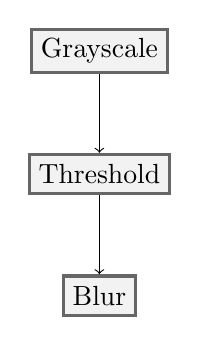
\begin{tikzpicture}[
		rectnode/.style={rectangle, draw=black!60, fill=black!5, very thick, minimum size=5mm},
	]

		% nodes
		\node[rectnode]	(gray) 								{Grayscale};
		\node[rectnode] (threshold) [below=of gray] 		{Threshold};
		\node[rectnode] (blur)  	[below=of threshold] 	{Blur};

		% lines
		\draw[->] (gray.south) -- (threshold.north);
		\draw[->] (threshold.south) -- (blur.north);

	\end{tikzpicture}
	\caption{The image pre-processing pipeline.}
	\label{fig:pre-processing}
\end{figure}

\section{Results}

\section{Conclusion}

\printbibliography

\end{document}
